\documentclass[../../AdvancementSummary.tex]{subfiles}

\begin{document}



%%%%%%%%%%%%%%%%%%%%%%%%%%%%%%%%%%%%%%%%%%%%%%%%%%%
\section{Results: Surface Effects}
%%%%%%%%%%%%%%%%%%%%%%%%%%%%%%%%%%%%%%%%%%%%%%%%%%%

Disordered proteins aid many reactions by acting as biological tethers. They may be permanent tethers tying two globular domains together or a domain to a surface \hl{example, example, cite cite}.  They may also be transient tethers, catching diffusing particles and tethering them to another molecule, i.e. formin. \hl{cite} By tethering molecules or surfaces together, disordered domains effectively increase the local concentration of a particle. This increases reaction rates by improving the probability of two molecules bumping into each other through restriction of their diffusive domain.

Given that a surface reduces the exploration space of a molecule, it will naturally increase the local concentration without a tether. However, it will also reduce the accessibility of a molecule by sometimes occluding, for example, an enzymatic domain from reaching its substrate in the correct orientation. Given that the surface has both positive and negative effects on reaction rates, how does being tethered to a surface impact a reaction compared to being tethered to a smaller domain? 

This type of interaction arises frequently with clustered reactions.  For instance, the phosphorylation of a membrane tethered disordered domain by a membrane bound kinase. \hl{cite} Experimental studies of such reactions are more easily performed on a sparse matrix such as dextran than on a hard surface. Therefore, it is important to understand the effect tethering to a surface has over tethering to a matrix. We explore how the presence of a surface influences the reach of a tethered domain and the overall local concentration.

\subsection{Presence of a surface restricts access to binding sites}


\hl{Pick one of these?}
\hl{make one figure in inkscape to control spacing}

\begin{figure}[H]
    \begin{center}
        \begin{subfigure}{\linewidth}
        		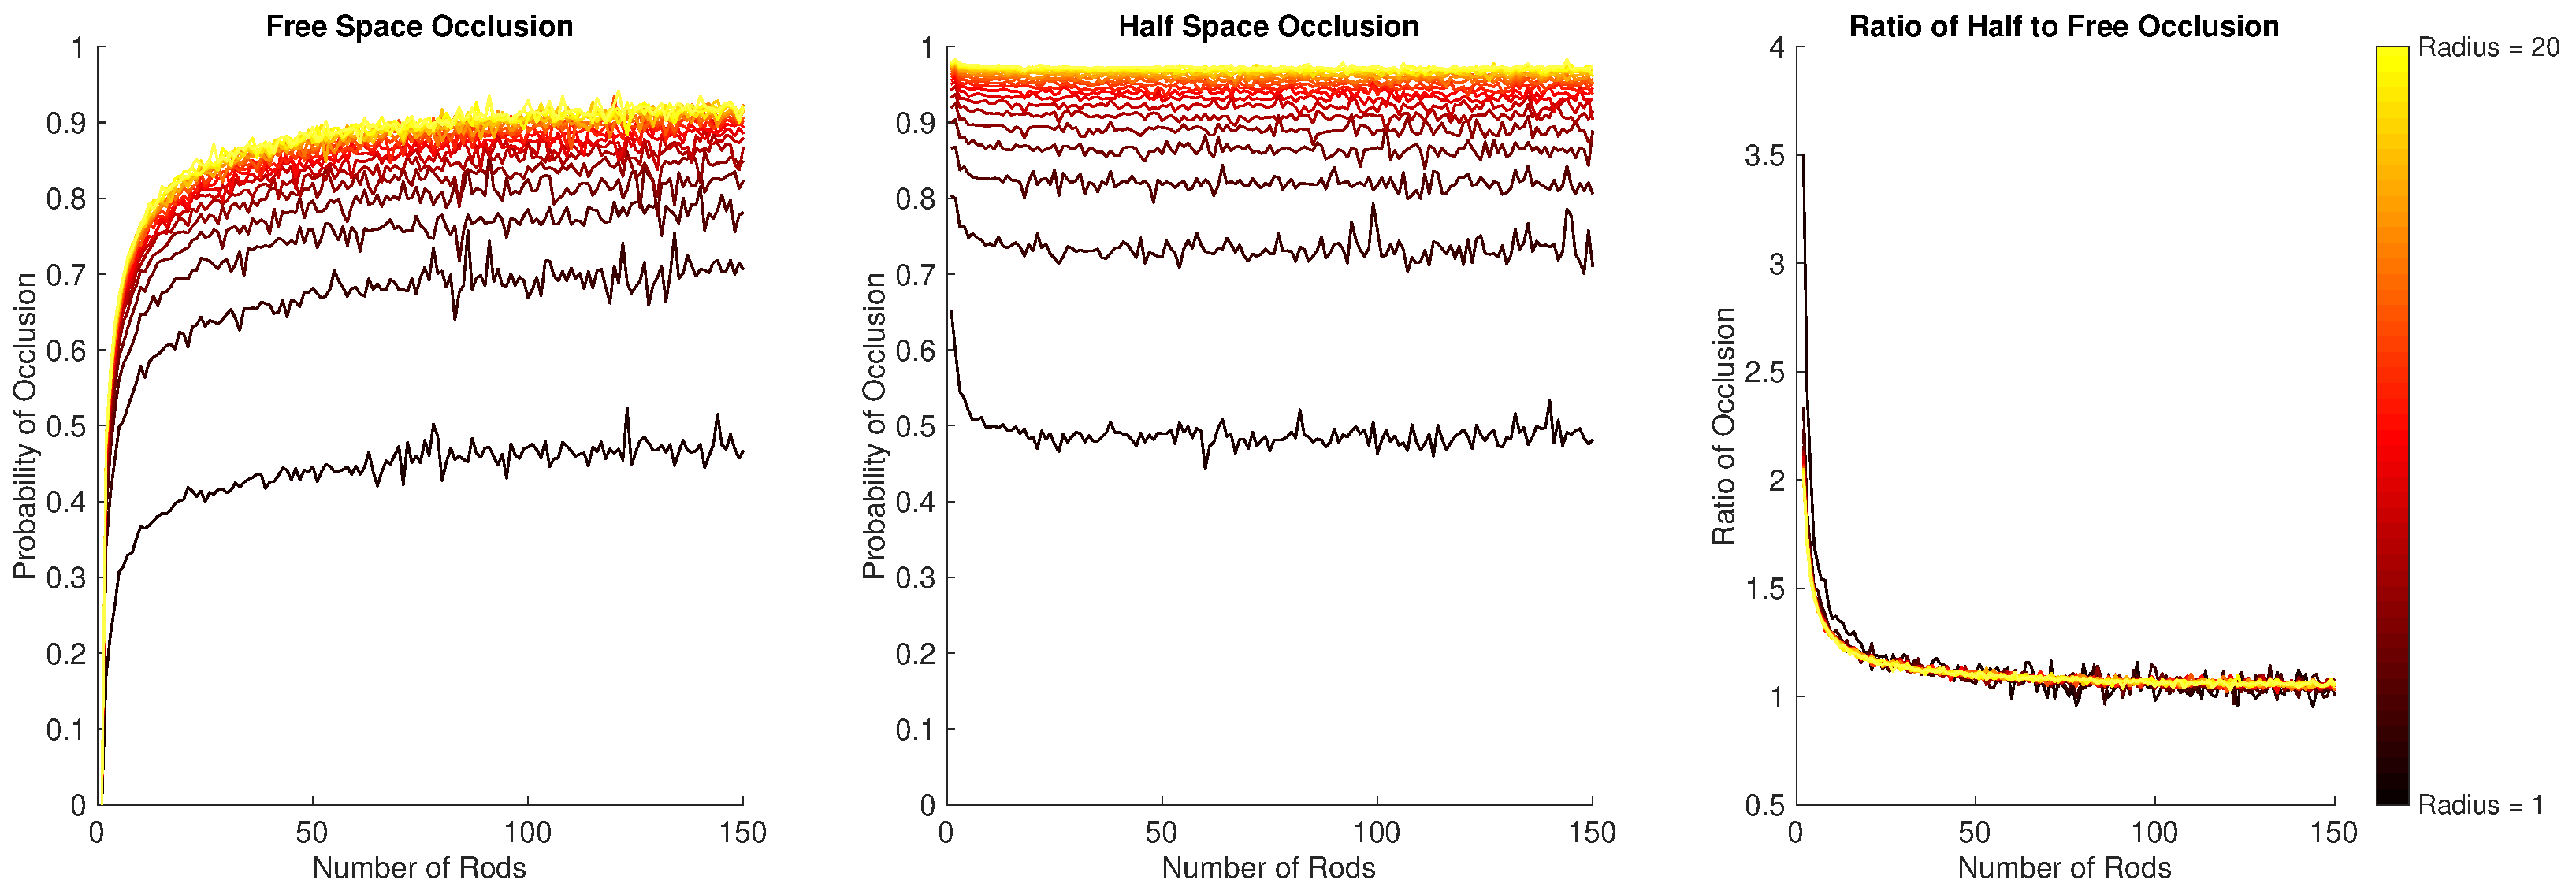
\includegraphics[width=\linewidth]{ResultsFigures/BindingSurfaceFactor/OcclusionVSN.eps}
        		\caption{}
        \end{subfigure}
        	\begin{subfigure}{\linewidth}
        		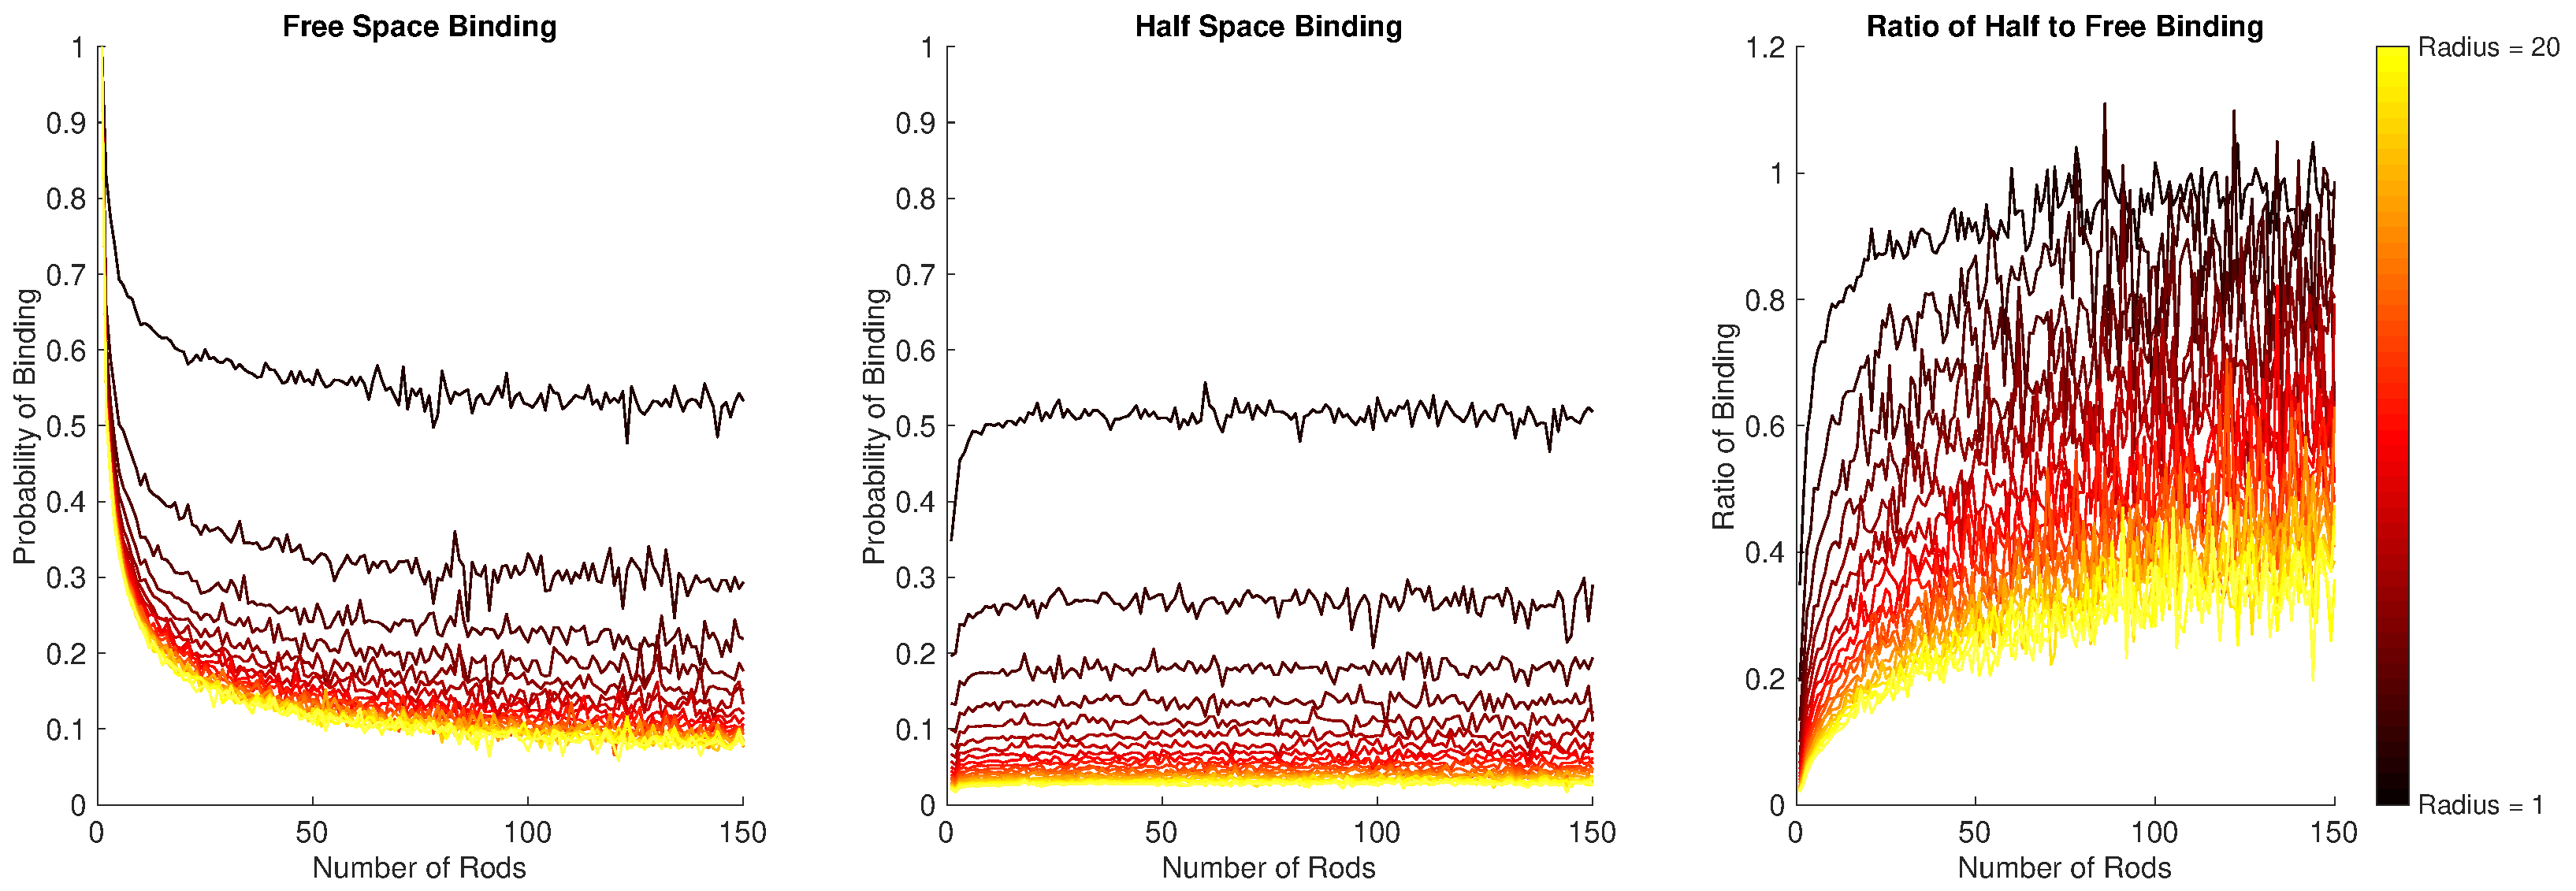
\includegraphics[width=\linewidth]{ResultsFigures/BindingSurfaceFactor/BindingVSN.eps}
        		\caption{}
        \end{subfigure}
        \caption{}
    \end{center}
\end{figure}

\subsection{SHP1}

\hl{Paragraph about SHP1}

\hl{reread SPR paper} 

\subsubsection{Model Tethers as Freely Jointed Chain}

We explore the effects of a surface on three different tethers, each modeled as a freely-jointed chain characterized by their lengths as measured in Kuhn lengths.  For each tether, we assume a Kuhn length,$\delta$, of 0.3nm, as supported by \hl{CITATION HERE}. Given that these tethers are made up of PEG linkers and amino acids, each of which is approximately the size of a Kuhn length, the lengths of each tether may be approximated as $N$ Kuhn lengths, where $N$ is the total number of PEG linkers and amino acids. Note that we consider the size of biotin to be negligible for our simulation.


%% Table of Tethers

\begin{center}
\begin{tabular}{| c | p{10cm} | c |}
	\hline
		Tether Name & Structure & N \\ 
		\hline 
		PD-1 	& 	(37392 B2) Bio-SRAARGTIGARRTGQPLKEDPSAVPVFSV
					DYGELDFQWREKTPEPPVPSVPEQTEY*ATIVFPSG 			& 	64	 \\
		PEG-3 	& 	Bio-(PEG)3-DLQEVTY*IQLDHH 							& 	16	 \\ 
		PEG-28 	& 	Bio-(PEG)28-DLQEVTY*IQLDHH 							& 	41	 \\
	\hline
\end{tabular}
\end{center}

\subsubsection{SHP1 Parameters}

We estimate the volume of SHP-1 based on its molecular weight, 67561$Da$,  as listed in UniProt entry P29350. We use an average protein density of 1.41$g/cm^3$ (Fischer et al. 2004 Protein Sci).

%\cite{UniProtSHP1} 
%\cite{FischerProteinSci2004}

\begin{equation*}
(67.5 \times 1000 \mbox{Da}) * (1.66\times10^{-27} \mbox{kg / Da}) * (1000 \mbox{g / kg}) / (1.41 \mbox{g / cm}^3) = 79.468 \nm^3.
\end{equation*}

If we then approximate the phosphatase domain as a sphere, then we can estimate a radius: 

\begin{align*}
V &= \frac{4}{3}\pi r^3 \\
79.468 \nm^3 &= \frac{4}{3} \pi r^3 \\
r &\approx 2.7 \nm \\
\end{align*}

For comparison, we also estimate an upper bound on the radius of SHP-1 from PyMol measurements of the SHP-1 structure (PDB 3PS5). Rounding up for measurement error, the longest part of the structure is 86 \AA. From this we calculate a maximum radius of 4.3$nm$.

\begin{figure}[H]
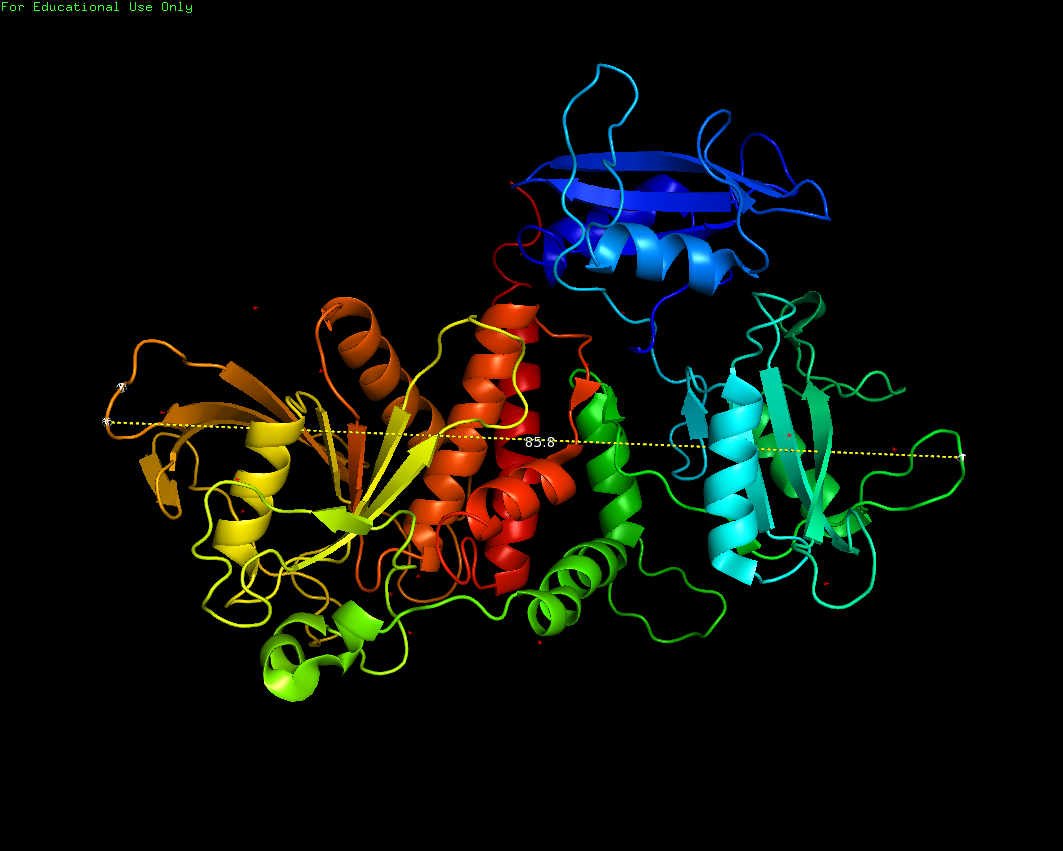
\includegraphics[width=\linewidth]{ResultsFigures/SHP1PyMol/Diagonal1.png}
\caption{Measurement of maximum length (in Angstroms) of SHP-1 (PDB 3PS5). }
\end{figure}

Alternatively, we can estimate the volume of SHP-1 as a rectangular prism and then create a spherical approximation of equal volume. We estimate the length, width and depth of SHP-1 to be 76\AA, 36\AA, and 58\AA respectively, giving a volume of 158688\AA$^3$.  From this, we calculate the radius for a spherical approximation to be 3.4nm.

\begin{figure}[H]
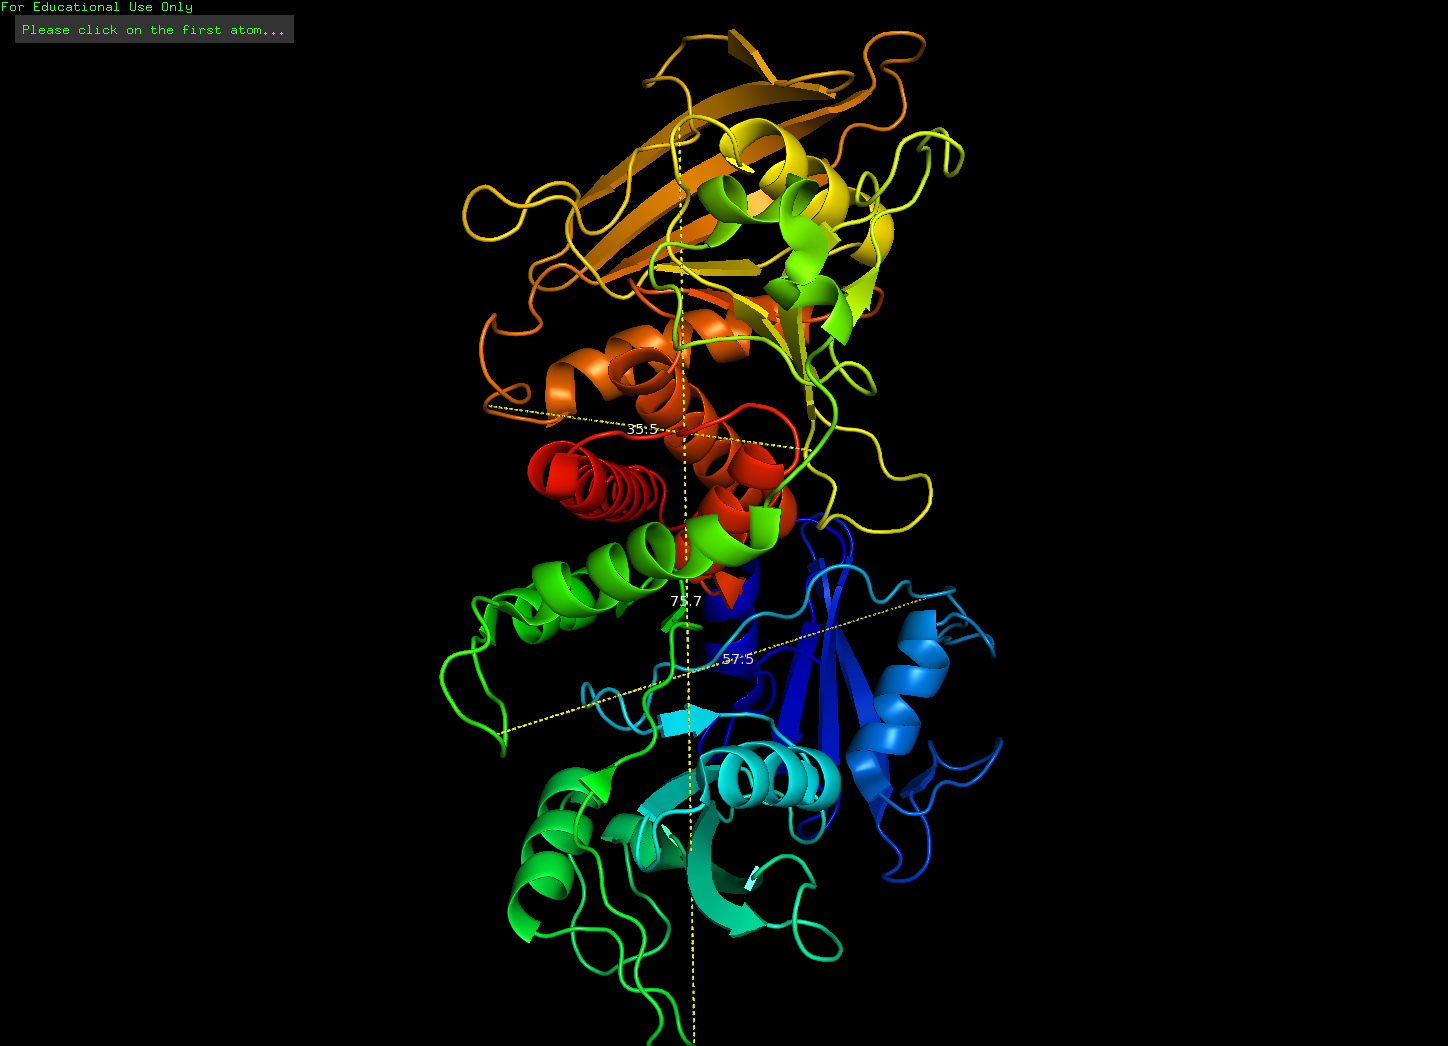
\includegraphics[width=\linewidth]{ResultsFigures/SHP1PyMol/LengthWidthDepth.png}
\caption{Measurement of rectangular dimensions (in Angstroms) of SHP-1 (PDB 3PS5).  }
\end{figure}


\subsubsection{Model Extension}
%% Goal

% description of simulation - polymer-c code
Using the parameters estimated above, we simulate two equivalent tethers in free-space and half-space.  The idealized SHP1 sphere, or ligand, is bound to the end of one of the tethers.  The second tether has a ghost ligand attached in the same location.  (Fig 3) We allow each tether to explore conformation space, at each conformation determining if the ghost ligand is occluded by the rest of the tether, or in half-space, by the half-space barrier. For the tether with the ghost ligand, we record both the location of the center of the ligand and whether or not it was occluded at each conformation.  For the tether with the bound ligand, we only record the location. 

% description of simulation - matlab code
The local concentration is alternately considered as the probability that the bound ligand is able to bind at the site of the ghost ligand within a small radius. \hl{I don't like this description}  To calculate this, we separate the the tethers from each other by a distance, $\rho$, measured in Kuhn lengths by adding $\rho$ to the $x$-coordinate of the ghost ligand. We then measure the distance between the two ligand centers, bound and ghost. If the centers are within a cutoff distance from each other AND the ghost sphere is not occluded, then the bound ligand is able to bind.  This is calculated as a probability, which is then converted to a local concentration by dividing by the volume of the sphere defined by the cutoff radius.

%% Diagram of simulation
\begin{figure}
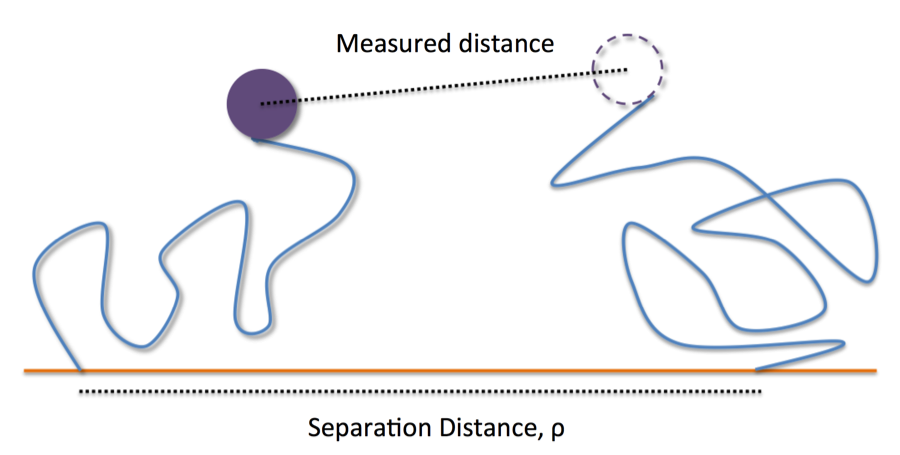
\includegraphics[width=\linewidth]{Diagram.png}
\caption{Cartoon of local concentration simulation in half space.}
\end{figure}



\subsubsection{Ligand radius and presence of a surface impact local concentration of tethered polymers}

We explore how effective concentration is impacted by ligand size and polymer length, where effective concentration is a description of how often a ligand bound to the end of one polymer encounters a binding site on the end of a second polymer, with the two polymers separated by some distance. When ligand size is zero, or equivalent to no ligand attached to the polymer, then we see the free space polymers experience an effective concentration predicted by the worm-like chain model. Note that variability from the theoretical WLC curve is mitigated by decreasing the cutoff considered local. \hl{weird wording} However, when we introduce a surface or ligand of nonzero size, the worm-like chain model no longer describes the effective concentration.  We see that the surface enhances the effective concentration over the free space values but that a larger ligand size reduces the effective concentration.

\hl{Should really use SHP1 parameters for this figure.}
\begin{figure}[H]
    \begin{center}
        		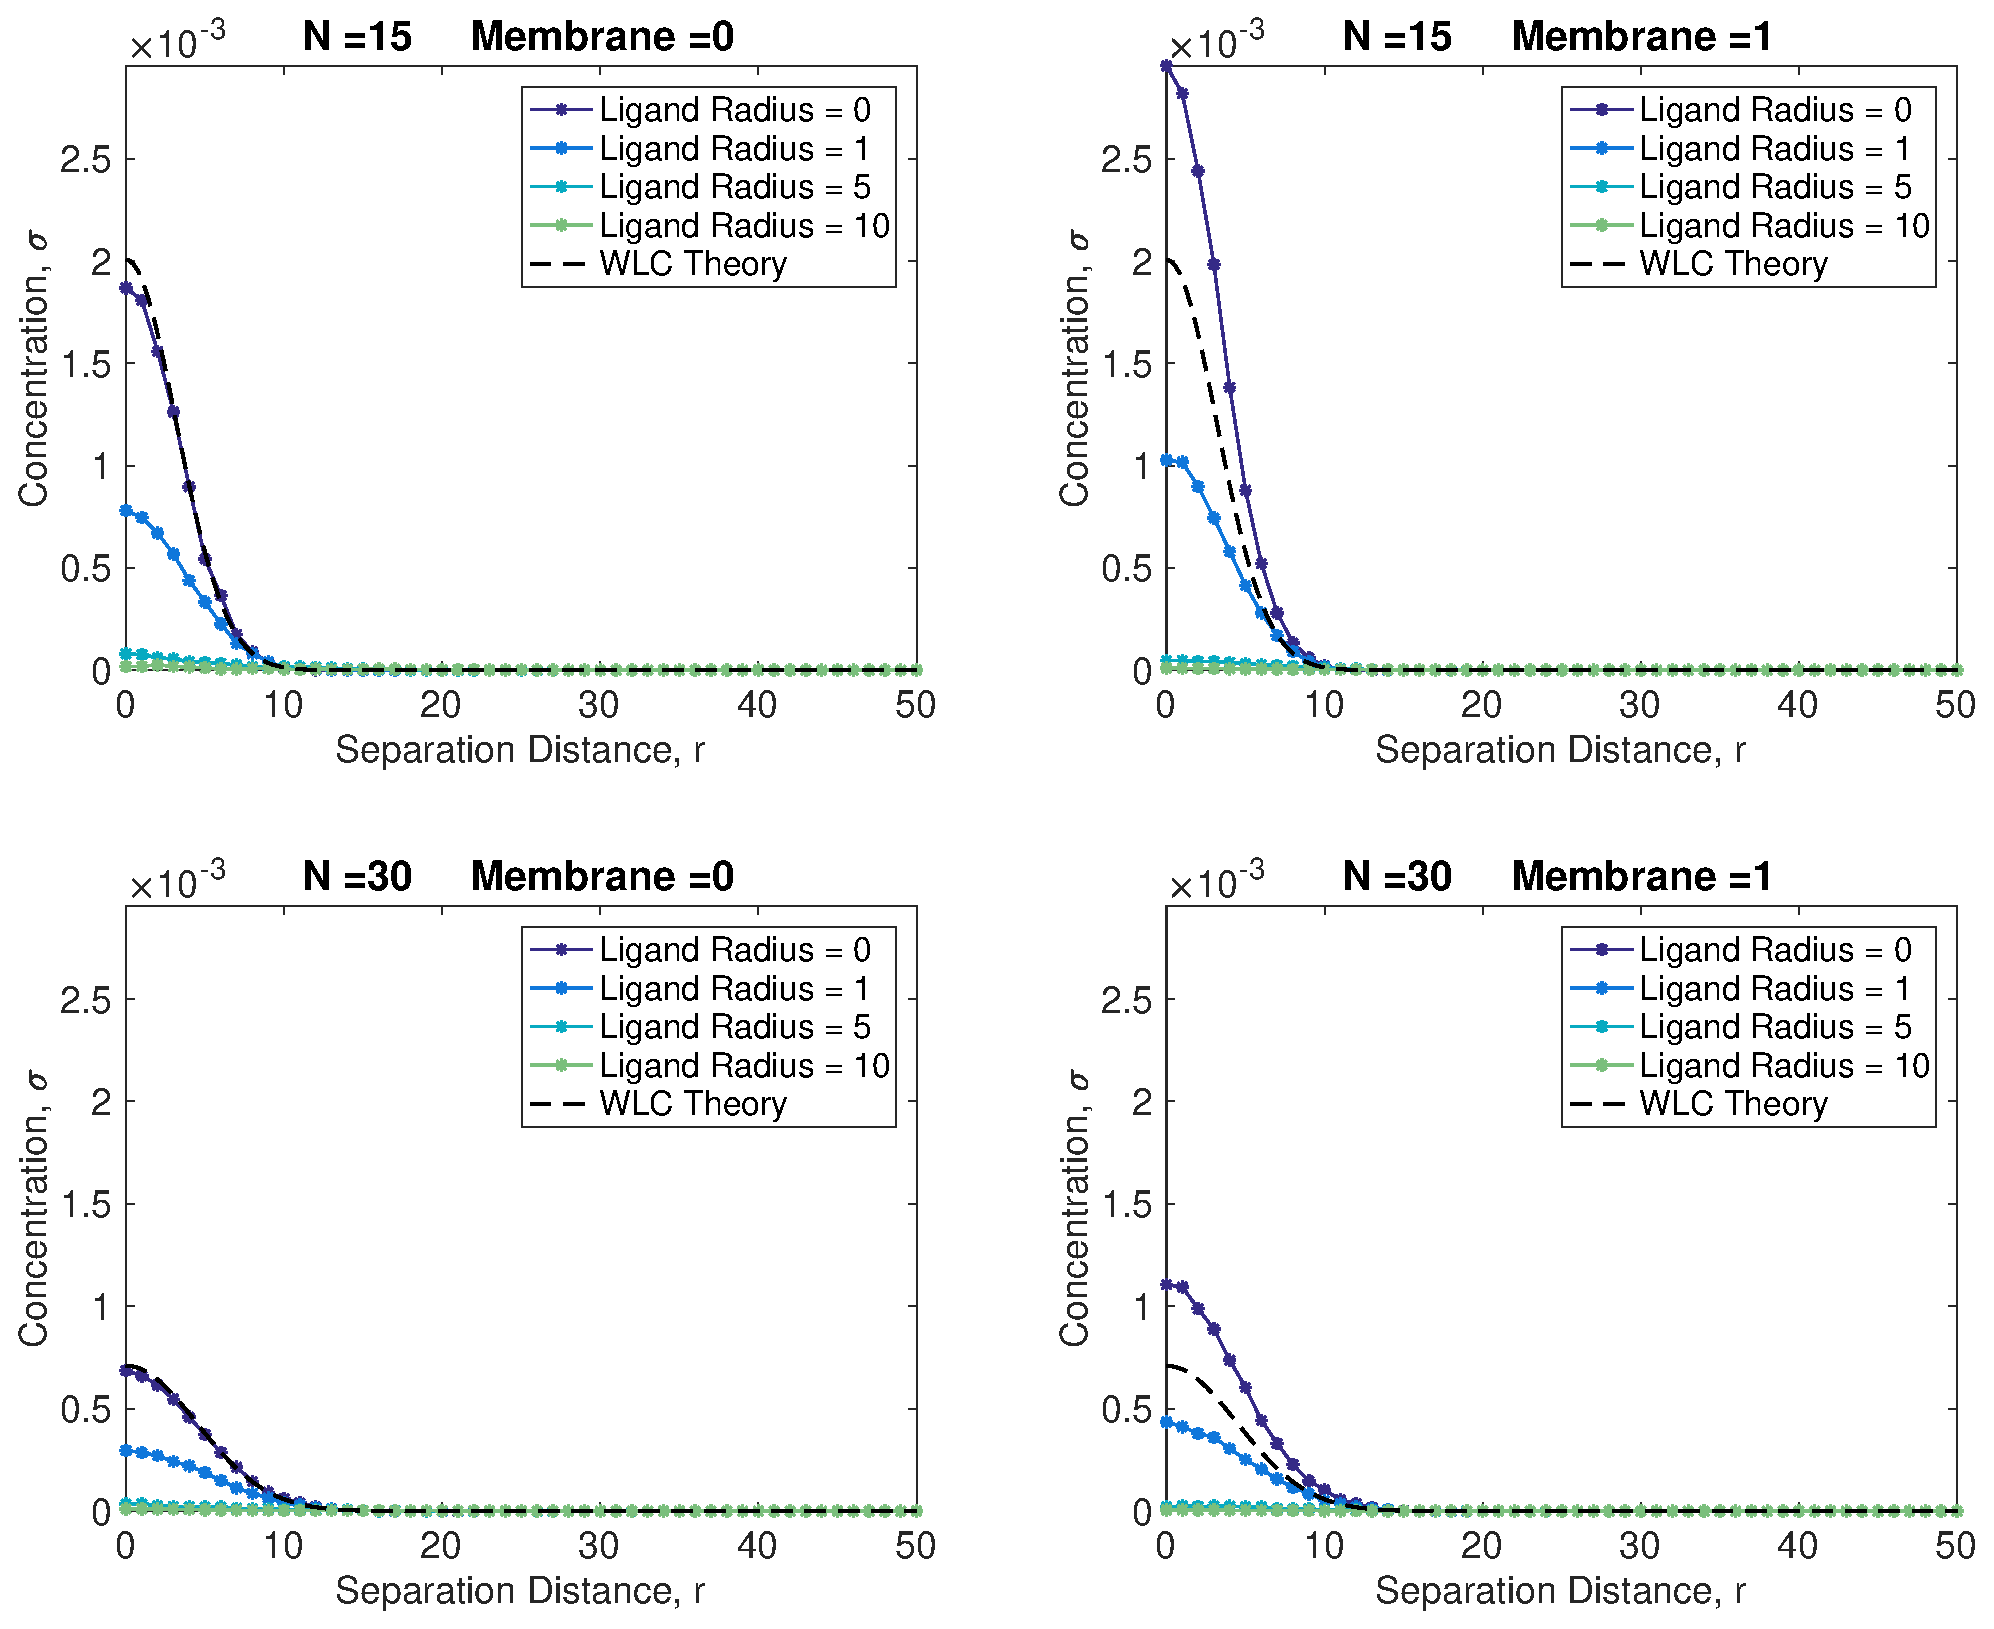
\includegraphics[width=0.8\linewidth]{ResultsFigures/EffectiveConcentrationKernel/ConcentrationVSSeparation.eps}
        \caption{}
    \end{center}
\end{figure}

\begin{figure}[H]
    \begin{center}
        		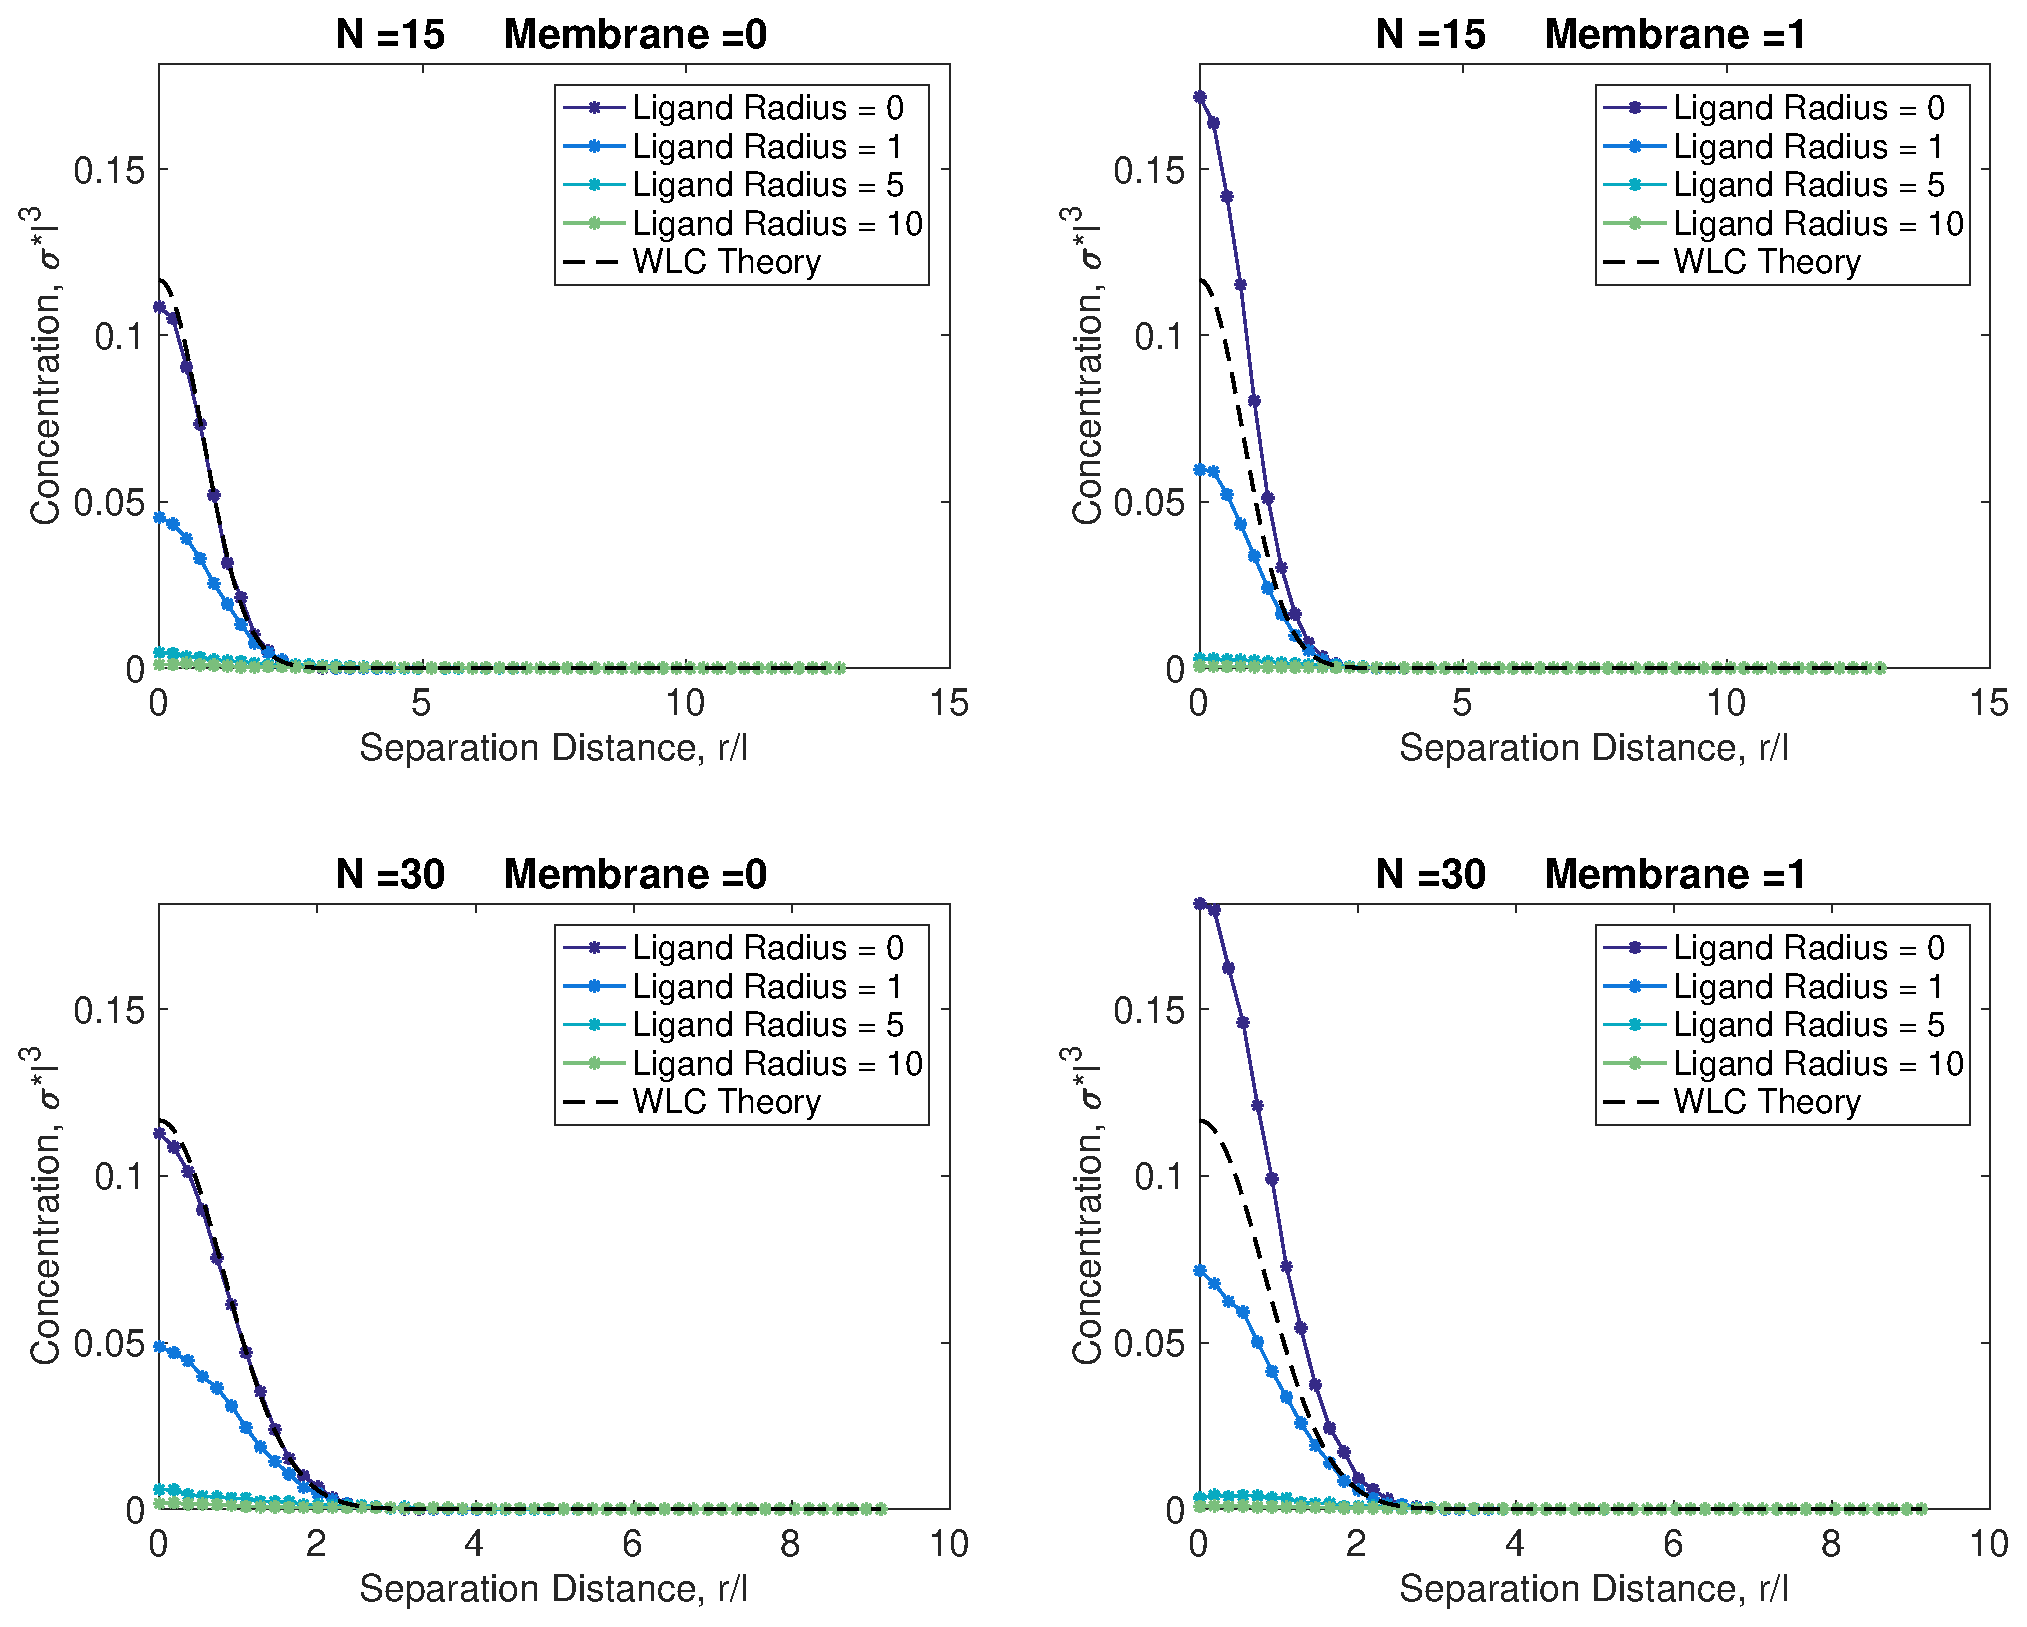
\includegraphics[width=0.8\linewidth]{ResultsFigures/EffectiveConcentrationKernel/ConcentrationNondimVSSeparation.eps}
        \caption{}
    \end{center}
\end{figure}


\subsubsection{Correction Factor}

The theoretical local concentration for two tethers a distance $\rho$ apart can be given by the following equation if both tethers are perfect worm-like chains:

\begin{equation}
	\sigma_{WLC}(\rho) = \left(\frac{3}{2\pi}\right)^{3/2} \frac{1}{L^3}e^{-\frac{3\rho^2}{2L^2}}
\end{equation}

Experimentally, we measure the reaction rate $R(\rho)$.  This equation is the product of a $k_{cat}$ and $\sigma(\rho)$.  If the two tethers were perfect worm-like chains and the attached ligand did not impact the local concentration then when we fit the experimental $R(\rho)$ to $\sigma_{WLC}(\rho)$, we would have $R(\rho) = k^{true}_{cat}*\sigma_{WLC}(\rho)$. However, since this is unlikely to be the case, if we fit to the WLC theory curve anyway, then we actually have $R(\rho) = k^{false}_{cat}*\sigma_{WLC}(\rho)$. Instead, if we consider our simulated data to be the true local concentration and we fit a half-gaussian curve, $\sigma_{fit}(\rho)$, to the data, then we would have $R(\rho) = k^{true}_{cat}*\sigma_{fit}(\rho)$, where $\sigma_{fit}(\rho) = a*e^{-\rho^2/c^2}$.

We can use the simulated data to give an estimate of how incorrect $k^{false}_{cat}$ is compared to $k^{true}_{cat}$. We'll call this ratio $\kappa_{cat}$. Since we measured $R(\rho)$ experimentally, we must have:

\todo{This doesn't look super pretty}

\begin{align*}
R(\rho) &= R(\rho) \\
k^{false}_{cat}*\sigma_{WLC}(\rho, L) &= k^{true}_{cat}*\sigma_{fit}(\rho, a, c) \\
\kappa_{cat} = \frac{k^{false}_{cat}}{k^{true}_{cat}} &= \frac{\sigma_{fit}(\rho, a, c)}{\sigma_{WLC}(\rho, L)} \\
\kappa_{cat} &= \frac{a*e^{-\rho^2/c^2}}{\left(\frac{3}{2\pi}\right)^{3/2} \frac{1}{L^3}e^{-\frac{3\rho^2}{2L^2}}} \\
\kappa_{cat} &= \frac{aL^3}{\left(\frac{3}{2\pi}\right)^{3/2}} \\
\kappa_{cat} &= \frac{a\left(\sqrt{\frac{3}{2}}c\right)^3}{\left(\frac{3}{2\pi}\right)^{3/2} } \\
\kappa_{cat} &= ac^3\pi^{3/2}\\
\end{align*}

if we \hl{assume? note?} $c^2 = \sqrt{\frac{2}{3}}L^2 \implies L = \sqrt{\frac{3}{2}}c$.

%summary table of possible fits to experimental data
\begin{center}
\begin{tabular}{| c | c | c |}
	\hline
		Model & Truth & Result \\ 
		\hline 
		Worm-like chain 	& 	T 	& 	$R(\rho) = k^{true}_{cat}*\sigma_{WLC}(\rho)$	 \\
		& & \\
		Worm-like chain 	& 	F 	& 	$R(\rho) = k^{false}_{cat}*\sigma_{WLC}(\rho)$	 \\ 
		& & \\
		Half-gaussian fit 	& 	T 	& 	$R(\rho) = k^{true}_{cat}*\sigma_{fit}(\rho)$	 \\
	\hline
\end{tabular}
\end{center}


We must therefore find appropriate $a$ and $c$ values for our half-gaussian fit in order to calculate the error.

\subsubsection{Curve Fitting}

\todo{Be consistent about $\sigma(r)$, $\rho$ etc.}

To fit a half-gaussian curve to the simulation data, we use both Matlab's lsqcurvefit and fminsearch functions to fit the function $\sigma_{fit}(\rho) = a*e^{-\rho^2/c^2}$ to the data. The lsqcurvefit function uses the Trust-Region-Reflective Least Squares Algorithm by default whereas fminsearch uses the Nelder-Mead simplex algorithm. \todo{Reference Lagarias et al. ?}  The Nelder-Mead algorithm provides parameters, aFit and cFit, that better fit the data compared to the Trust-Region-Reflective Least Squares Algorithm. When we run a parameter sweep to heuristically determine if these are the optimal parameters, we find that the sum of least squares obtain using $aFit$ and $cFit$ is consistently lower than that of the lowest found with any of our sweep parameters.  Additionally, when we use the parameters which minimize the sum of least squares from our sweep to initialize the fminsearch function, our fit parameters change minimally and the sum of least squares differs by less than $10^{-10}$. For simplicity, we therefore use the fit parameters obtained from the Nelder-Mead algorithm.

\todo{clean up the language - too many fit parameters.  Is it ok to reference them by function name vs algorithm name?}


\subsubsection{Reach parameter is unaffected by presence of surface}

Our data shown earlier indicates that the presence of a surface will stretch a polymer compared to in free space. We would expect this straightening to also increase the reach parameter for the effective concentration. When we fit a half-gaussian curve to the simulated effective concentration curves, we find that the reach parameter, c, is unaffected by the presence of a surface. This parameter changes based on polymer length and ligand size, but is not impacted by a surface. 


\hl{include curve fitting figure?}

\begin{figure}[H]
    \begin{center}
        		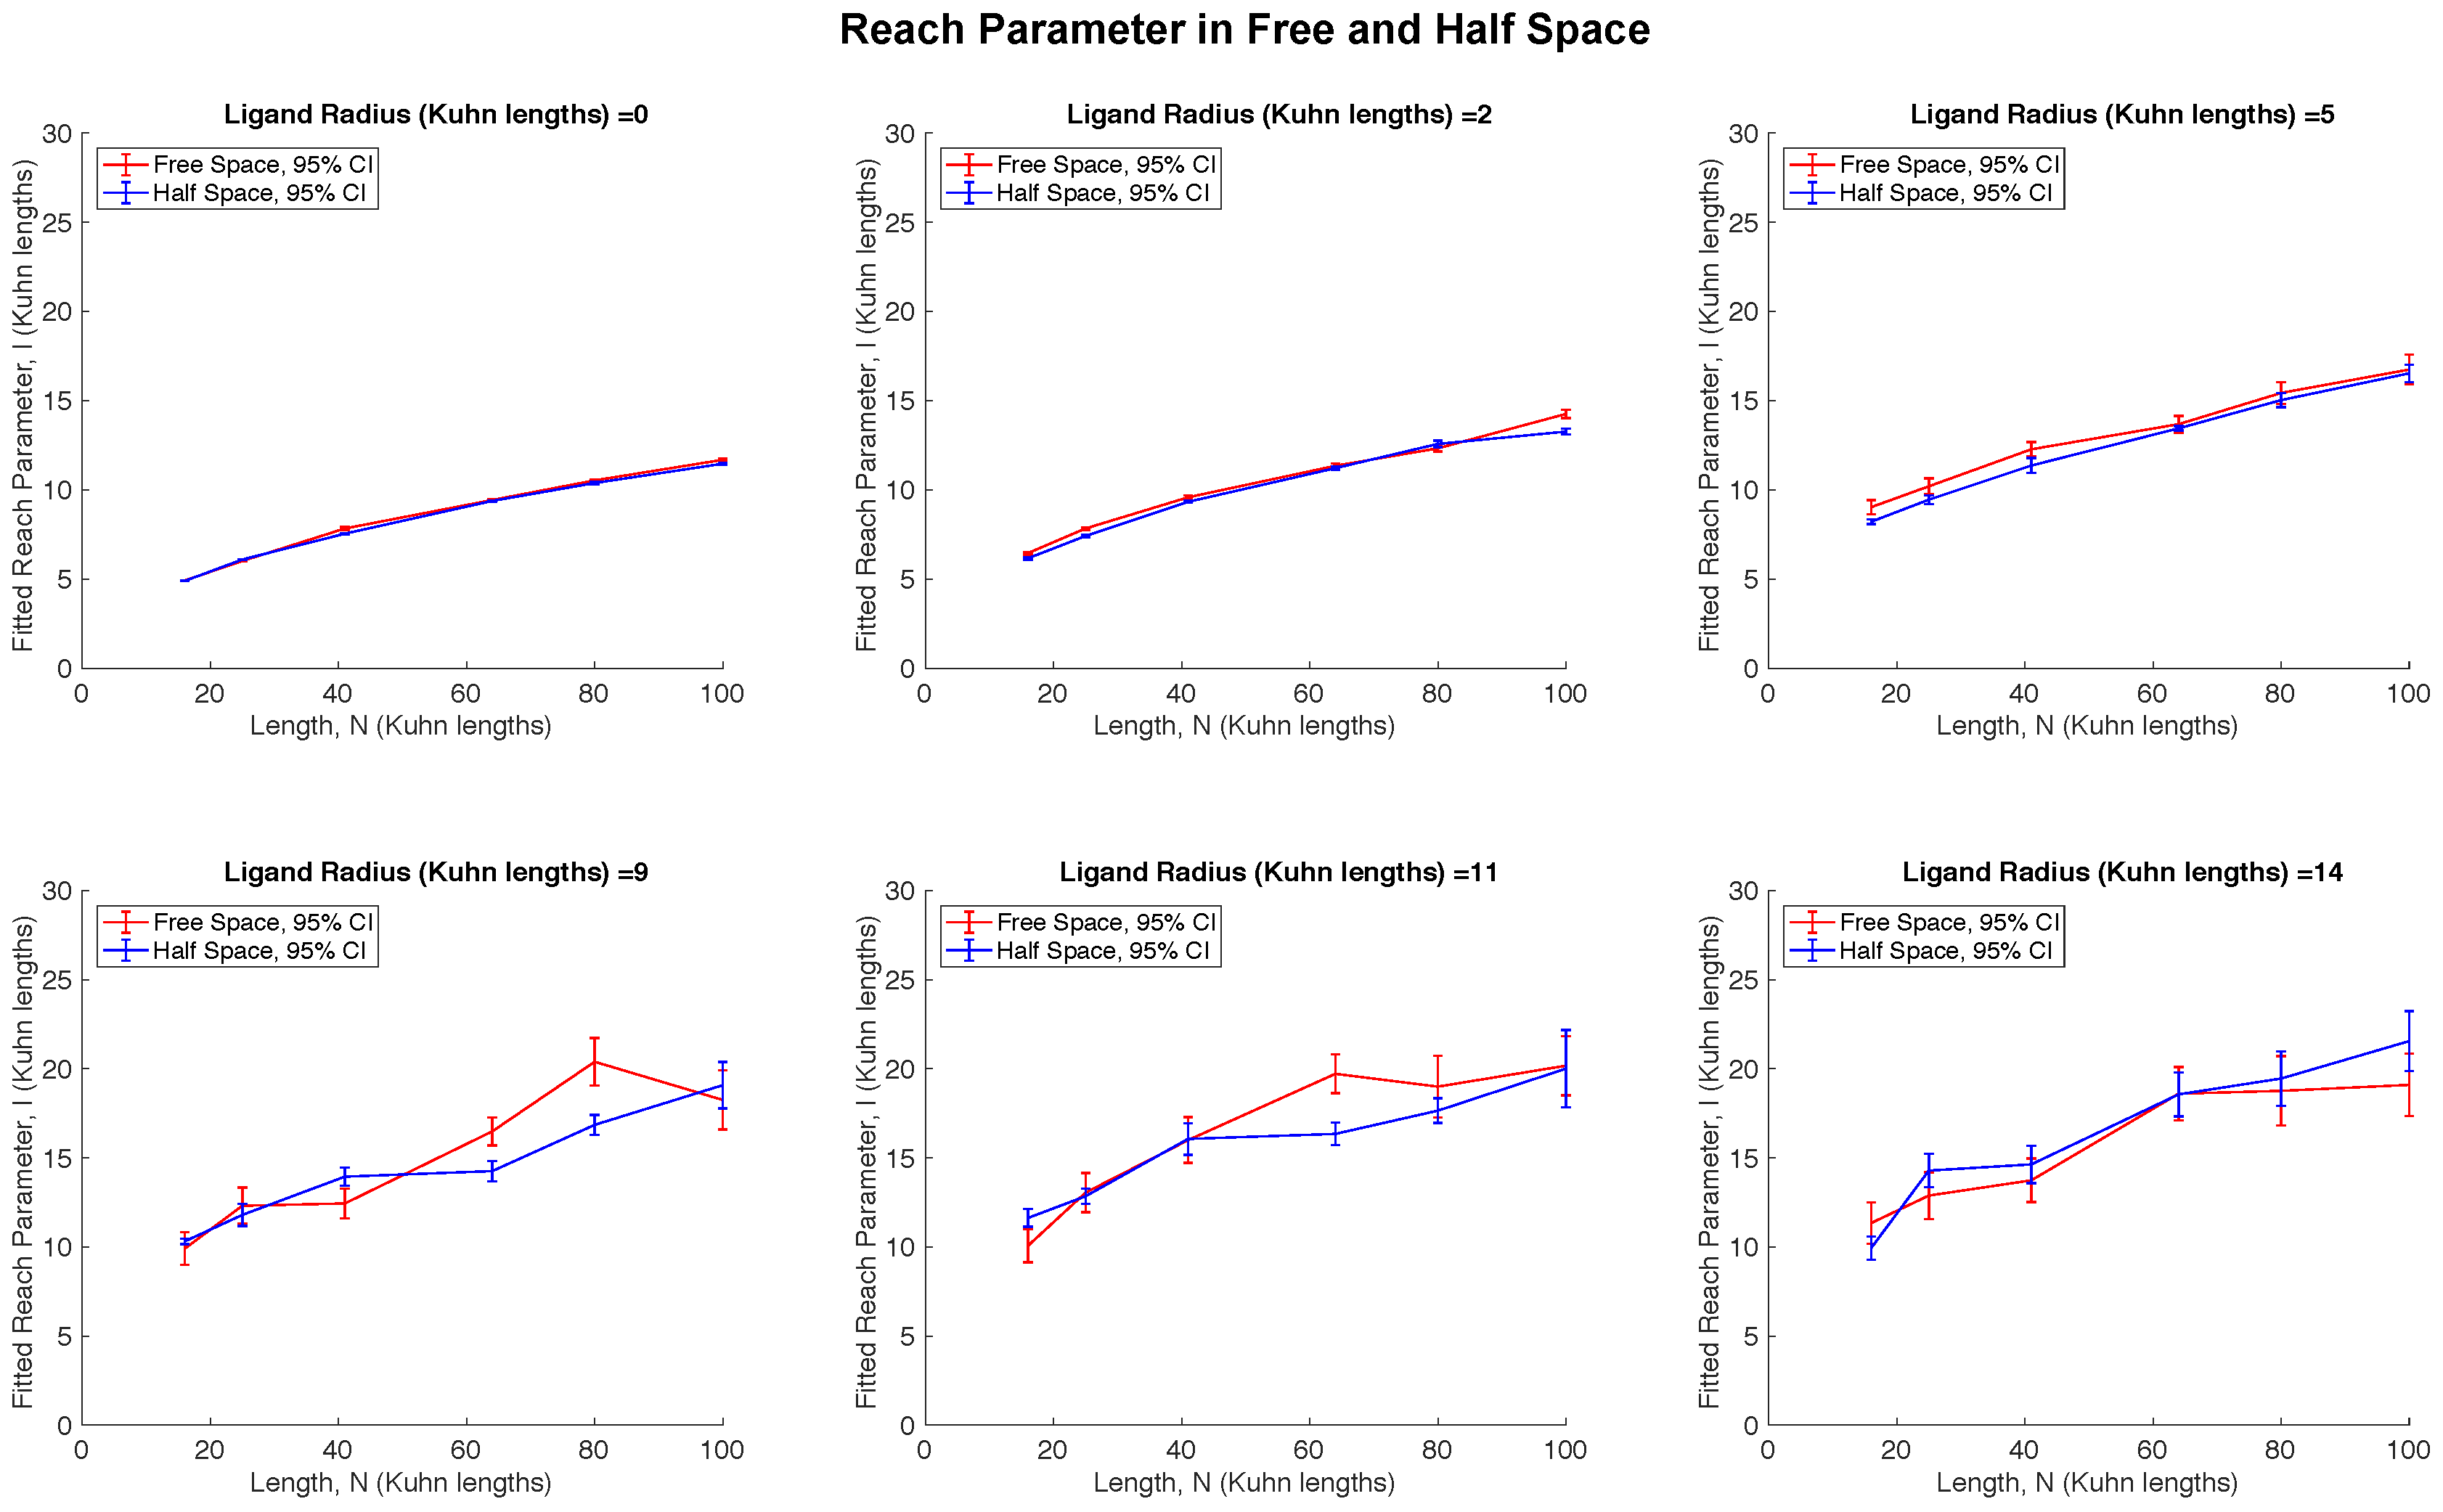
\includegraphics[width=\linewidth]{ResultsFigures/ReachSurfaceFactor/ReachParameterFreeHalfAxisEqual.eps}
        \caption{}
    \end{center}
\end{figure}

\begin{figure}[H]
    \begin{center}
        		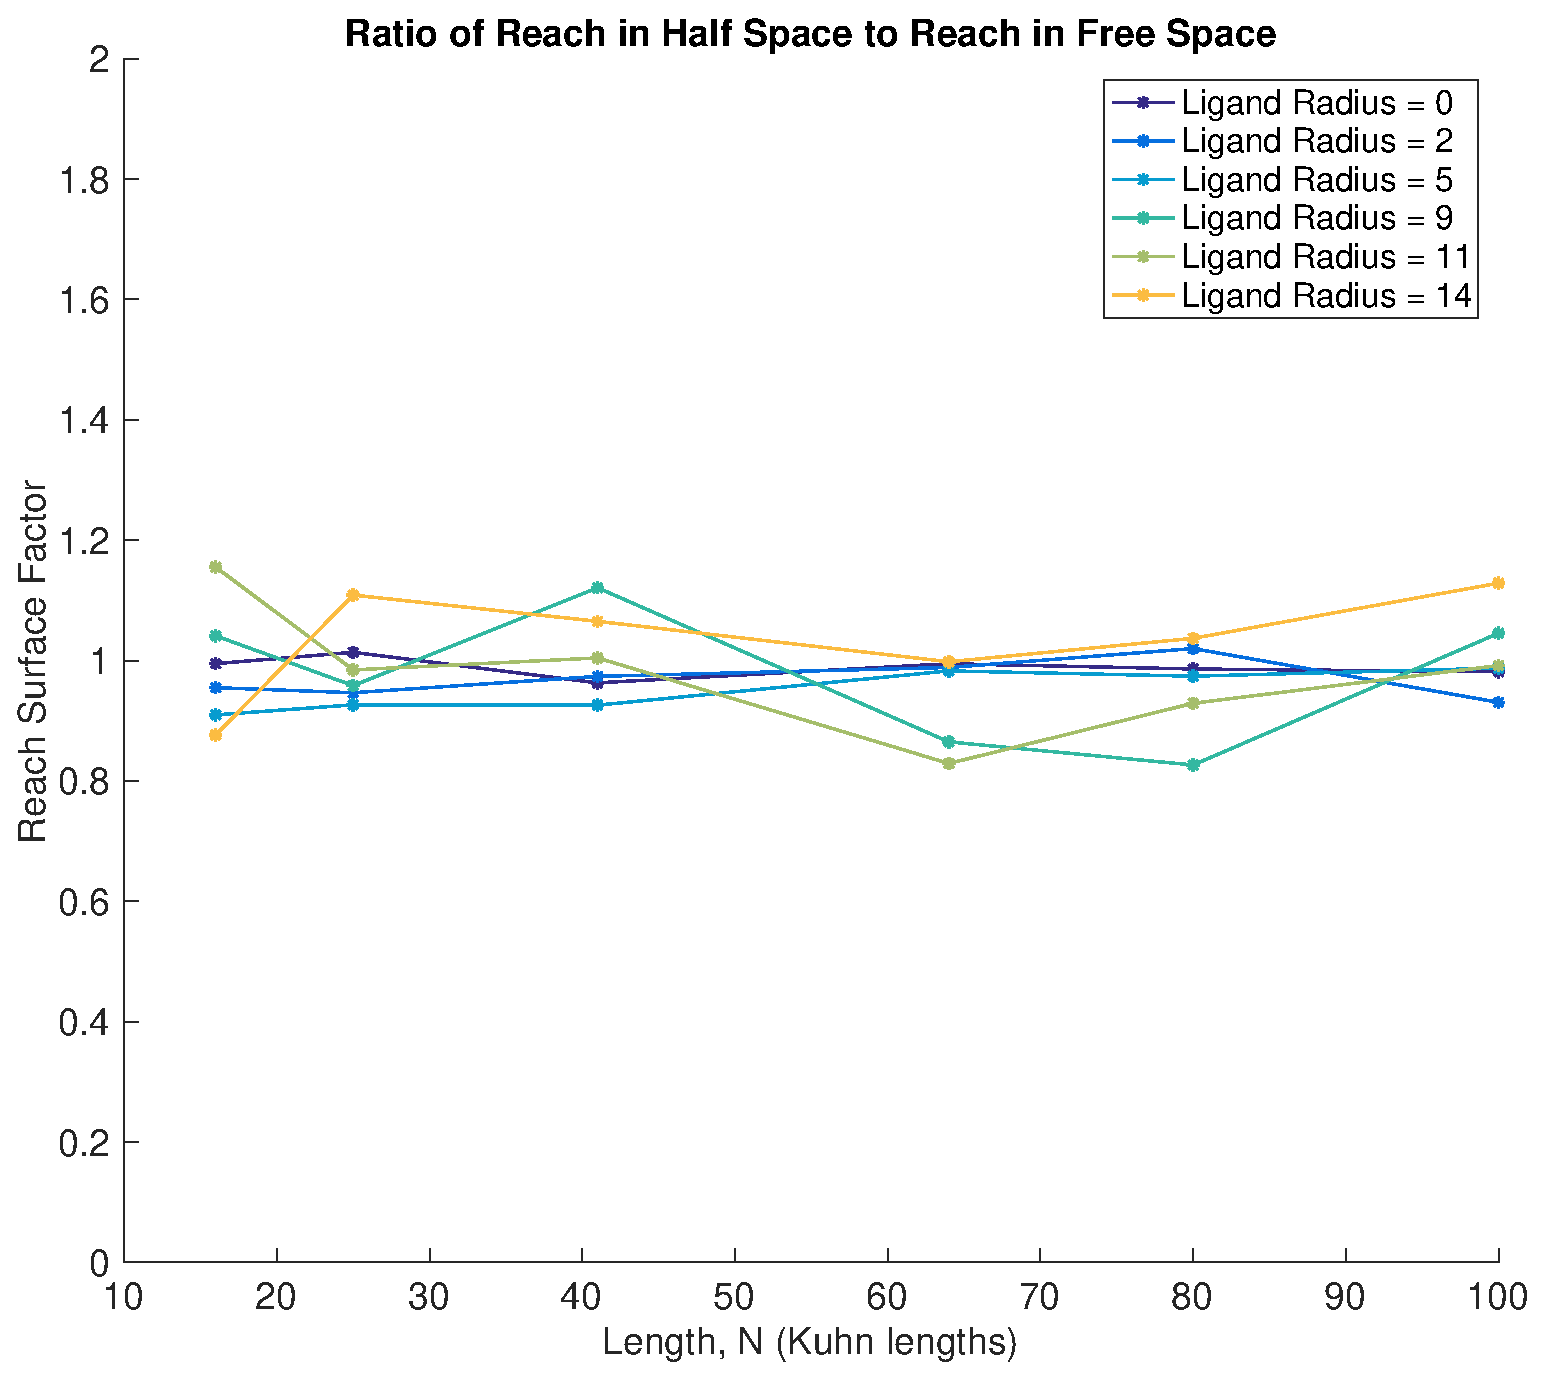
\includegraphics[width=0.7\linewidth]{ResultsFigures/ReachSurfaceFactor/ReachSurfaceFactor.eps}
        \caption{}
    \end{center}
\end{figure}


\subsubsection{Future Work}

Experimental measurements of effective concentration do not distinguish between the effective concentration and the catalytic rate. Since these values are lumped into a single number, it is important to know how the surface impacts the apparent catalytic rate.  \hl{This might be flat out incorrect.} \hl{ include calculation of how to find catalytic ratio?} We will plot the ratio of apparent catalytic rates for various polymer lengths and ligand sizes. This will indicate if there is a relationship between the catalysis factor and the reaction parameters or if there is a single value describing the impact of the surface. The catalysis surface factor may then be used to determine how experiments on a surface differ from on a matrix and possibly give a conversion factor between the two.









%%%%%%%%%%%%%%%%%%%%%%%%%%%%%%%%%%%%%%%%%%%%%%%%%%%
\end{document}
%%%%%%%%%%%%%%%%%%%%%%%%%%%%%%%%%%%%%%%%%%%%%%%%%%%





